% compile with
%      pdflatex -shell-escape diagram

\documentclass{article}
\usepackage[paperheight=6cm,paperwidth=12cm,margin=0cm]{geometry}
\usepackage{tikz}
\usetikzlibrary{calc}

\pagestyle{empty}

\begin{document}

  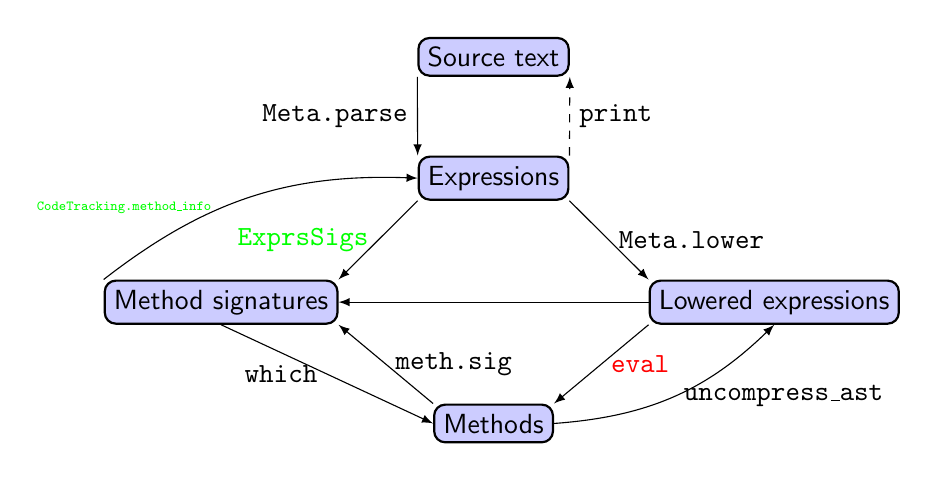
\begin{tikzpicture}[
      font=\sffamily,
      every matrix/.style={ampersand replacement=\&,column sep=1cm,row sep=1cm},
      object/.style={draw,thick,rounded corners,fill=blue!20},
      to/.style={->,shorten >=1pt,semithick,font=\sffamily\footnotesize},
      ]
      % every node/.style={align=center}]

    % Position the nodes
    \matrix{
      \& \node[object] (src) {Source text}; \& \\
      \& \node[object] (exprs) {Expressions}; \& \\
      \node[object] (sigts) {Method signatures}; \& \& \node[object] (lowered) {Lowered expressions}; \\
      \& \node[object] (methods) {Methods}; \& \\
    };

    % Draw the arrows and labels
    %\draw[to] (src) -- node[midway,left] {\texttt{Meta.parse}} (exprs);
    %\draw[to] (exprs) -- node[midway,right] {\texttt{print}} (src);
    \path [-latex] (src.south west) edge node[midway,left] {\texttt{Meta.parse}} (exprs.north west);
    \path[dashed] [-latex] (exprs.north east) edge node[midway,right] {\texttt{print}} (src.south east);

    \path [-latex] (exprs.south east) edge node[midway,right] {\texttt{Meta.lower}} (lowered.north west);
    \path [-latex] (lowered.south west) edge node[midway,right,color=red] {\texttt{eval}} (methods.north east);
    \path [-latex] (methods.east) edge [bend right=20] node[midway,right] {\texttt{uncompress\_ast}} (lowered.south);
    \path [-latex] (methods.north west) edge node[midway,right] {\texttt{meth.sig}} (sigts.south east);
    \path [-latex] (sigts.south) edge node[midway,left] {\texttt{which}} (methods.west);

v    \path [-latex] (exprs.south west) edge node[midway,left,color=green] {\texttt{ExprsSigs}} (sigts.north east);
    \path [-latex] (lowered.west) edge (sigts.east);

%    \path[dashed] [-latex] (methods.south west) edge [bend left=100] node[pos=0.75,left] {file,line} (src.west);
    %\draw[dashed,->] (methods) to[out=180,in=-90] ($(sigts)-(2,0)$) to[out=90,in=180] node[midway,left] {file,line} (src);
    \path [-latex] (sigts.north west) edge [bend left=20] node[pos=0.4,left,color=green] {\texttt{\tiny CodeTracking.method\_info}} (exprs.west);

  \end{tikzpicture}

  Base \qquad {\color{red} Base destructive} \qquad {\color{green} Revise}

\end{document}
